 
  The matrix method is valid under the assumption that the shapes of $p_{\mrm{Q}}(x)$ and $p_{\mrm{G}}(x)$ remain consistent, regardless of whether the jets are situated in the central or forward regions. Jet fragmentation at a $pp$ collider is expected to be predominantly influenced by the jet \pt~and is generally considered independent of $\eta$, considering the underlying parton type. Consequently, an approach aimed at extracting distributions associated with the radiation patterns of quark-jets and gluon-jets should be valid at the particle level. At the detector level, however, the measured radiation pattern within jets no longer retains its $\eta$-independence. This is due to variations arising from differences in detector materials and technologies, leading to distinctions between the central and forward regions in terms of response. As a consequence of these effects, the matrix method experiences deviations from closure,, indicating a disparity between the expected and actual outcomes.
  


The distributions of {\ntrk} have been seen to have systematic difference for the truth-labelled quark/gluon jets in the quark-enriched and gluon-enriched regions in each \pt~bin. To rectify this discrepancy and ensure alignment in the distribution of jet tagging variables between the central and forward regions, a re-weighting procedure is implemented. This procedure involves applying adjustments to account for the observed differences.  For each event, the central jet is weighted by a re-weighting factor :
\begin{equation}
%w_{\mrm{Q/G}}({x;p_{\text{T,j}}}) = \frac{ p_{\mrm{Q/G,~higher \abseta}}({x;p_{\text{T,j}}}) }{ p_{\mrm{Q/G,~lower \abseta}}({x;p_{\text{T,j}}})}
w_{\mathrm{Q} / \mathrm{G}}\left(x ; p_{\mathrm{T}, \mathrm{j}}\right)=\frac{p_{\mathrm{Q} / \mathrm{G}, \text { forward }}\left(x ; p_{\mathrm{T}, \mathrm{j}}\right)}{p_{\mathrm{Q} / \mathrm{G}, \text { central }}\left(x ; p_{\mathrm{T}, \mathrm{j}}\right)}
\label{eq:QG-reweight}
\end{equation}
where $q/g$ tagging variable $x$ is calculated in each jet \pt~bin for quark and gluon jets, respectively. By default the re-weighting factor derived from truth-labelled quark-jets is implemented for both types of jets, whereas the re-weighting factor derived from truth-labelled gluon-jets is used as an alternative to evaluate the systematic uncertainty from the re-weighting procedure, known as MC non-closure systematic uncertainty for the calibration.



The distributions of \ntrk~in extracted pure quark- and gluon-jets and truth-labelled MC before re-weighting as shown in Figure~\ref{fig:QG-pythia-NtrkMCExtractedNoReweight-Ntrk}. After the re-weighting the distributions of \ntrk~are shown in Figure~\ref{fig:QG-pythia-NtrkMCExtractedQuarkFactor-Ntrk}. The non-closure is at few percent level and is is taken as MC non-closure systematic uncertainty. 

\begin{figure}[htb]
	\centering
	\subfloat[ ]{\label{fig:QG-pythia-QuarkNtrkMCExtractedNoReweight-500-600-Ntrk}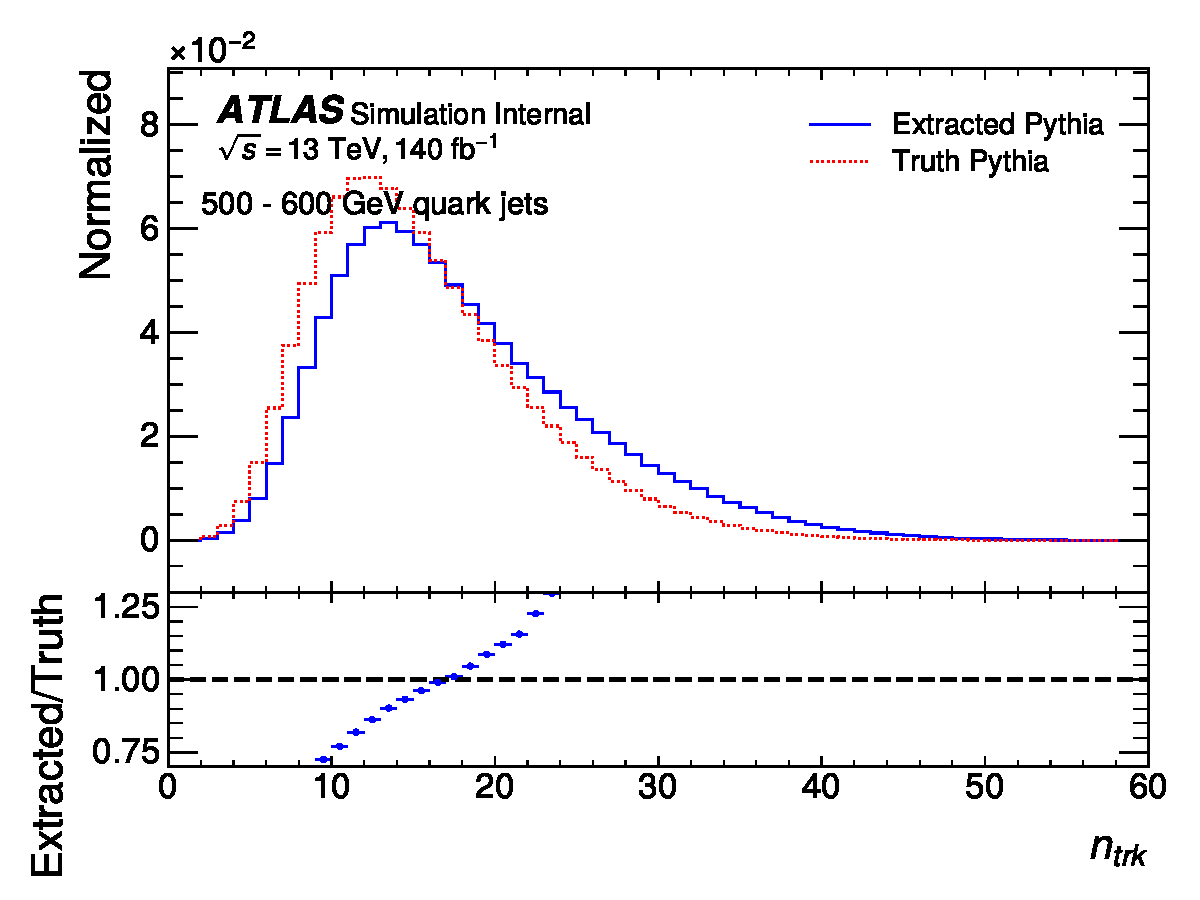
\includegraphics[width=0.45\textwidth]{fig/ADE/MCClosure/none_event_weight/jet_nTracks/MCClosure_500_quark_jet_nTracks.pdf}} \quad
	\subfloat[ ]{\label{fig:QG-pythia-GluonNtrkMCExtractedNoReweight-500-600-Ntrk}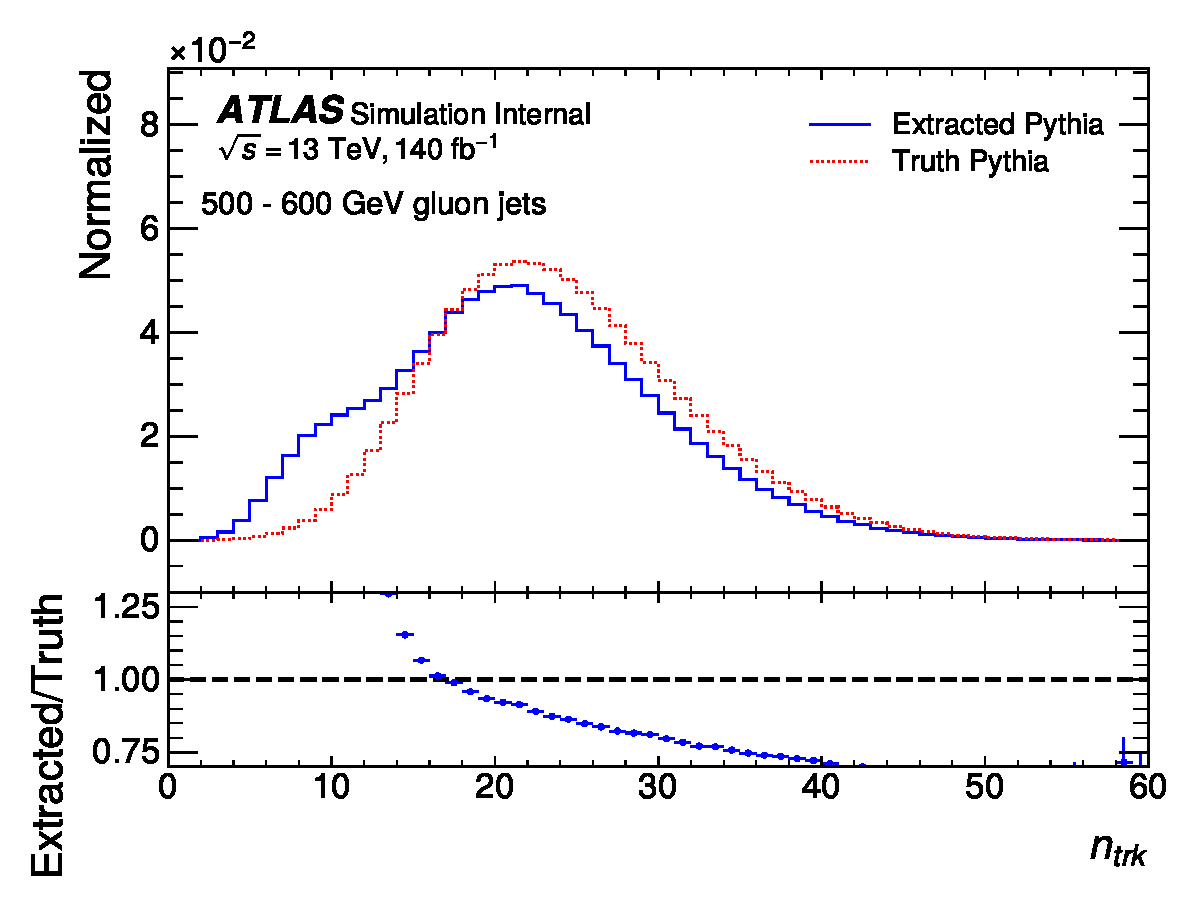
\includegraphics[width=0.45\textwidth]{fig/ADE/MCClosure/none_event_weight/jet_nTracks/MCClosure_500_gluon_jet_nTracks.pdf}} \\
	\subfloat[ ]{\label{fig:QG-pythia-QuarkNtrkMCExtractedNoReweight-800-1000-Ntrk}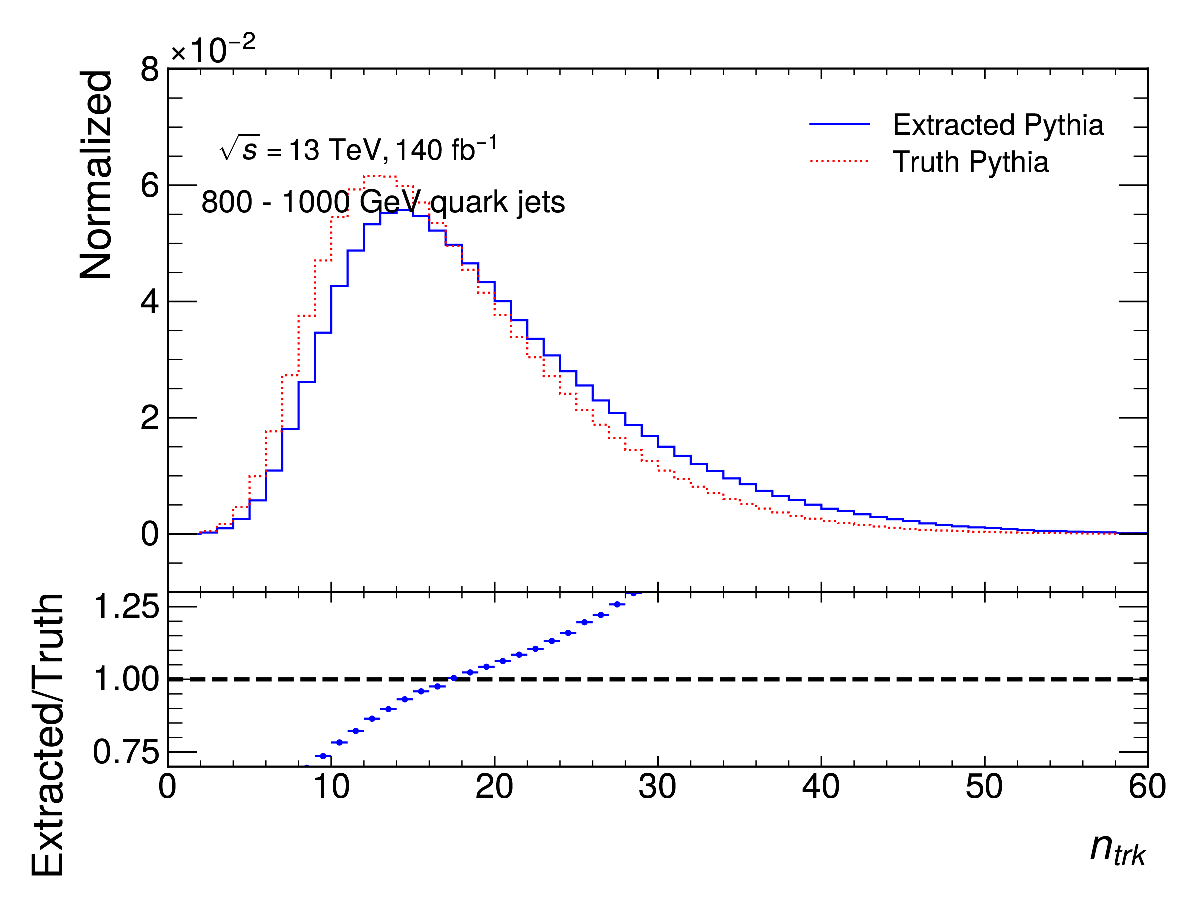
\includegraphics[width=0.45\textwidth]{fig/ADE/MCClosure/none_event_weight/jet_nTracks/MCClosure_800_quark_jet_nTracks.pdf}} \quad
	\subfloat[ ]{\label{fig:QG-pythia-GluonNtrkMCExtractedNoReweight-800-1000-Ntrk}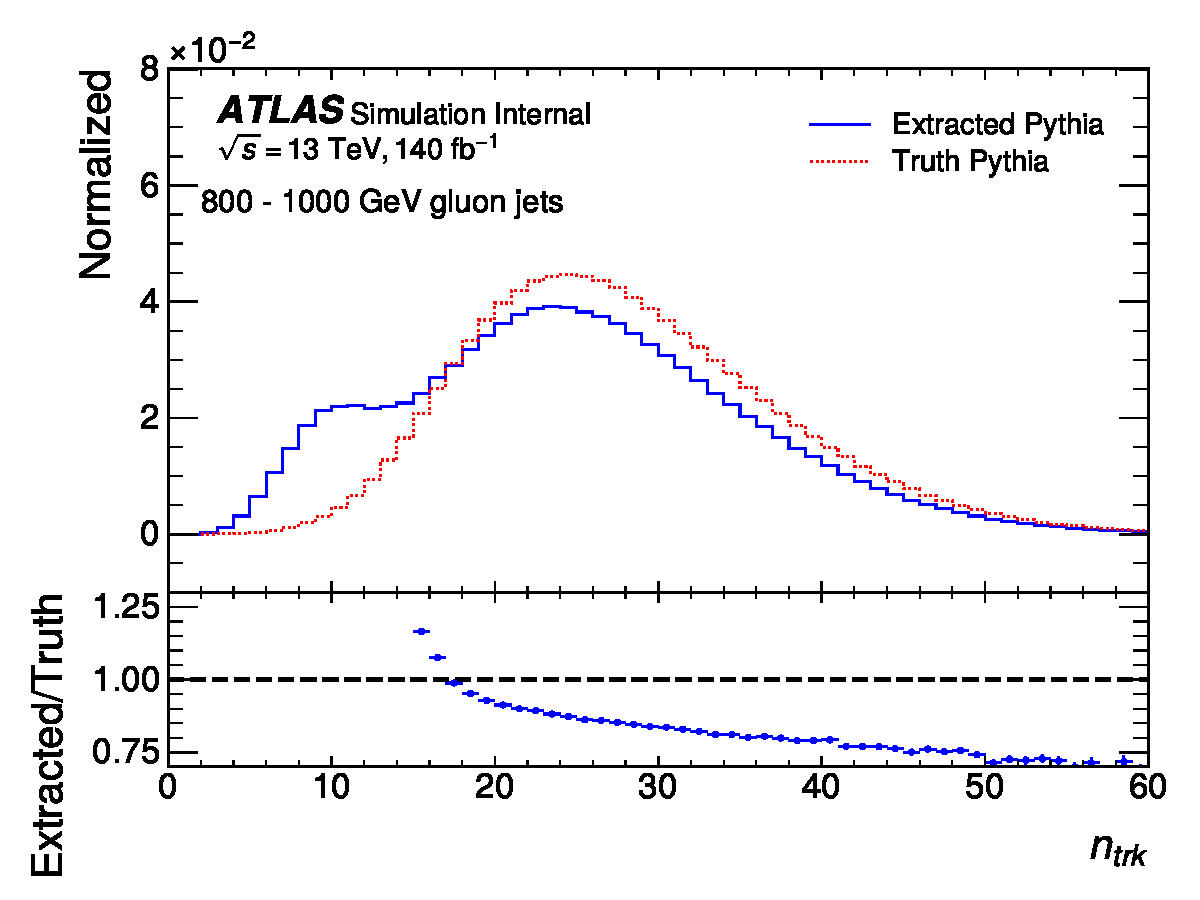
\includegraphics[width=0.45\textwidth]{fig/ADE/MCClosure/none_event_weight/jet_nTracks/MCClosure_800_gluon_jet_nTracks.pdf}} \\
	\caption[]{
		Before re-weighting: the {\ntrk} distributions of quark-jet \subref{fig:QG-pythia-QuarkNtrkMCExtractedNoReweight-500-600-Ntrk}  \subref{fig:QG-pythia-QuarkNtrkMCExtractedNoReweight-800-1000-Ntrk} 
		and  gluon-jet in \subref{fig:QG-pythia-GluonNtrkMCExtractedNoReweight-500-600-Ntrk}  \subref{fig:QG-pythia-GluonNtrkMCExtractedNoReweight-800-1000-Ntrk} 
		 from {\pythia8} sample. %
		Dashed and solid-line show the {\ntrk} distributions in the truth MC and extracted MC, respectively.
		Bottom panels show the ratio of the extracted MC to the truth MC. %
		\label{fig:QG-pythia-NtrkMCExtractedNoReweight-Ntrk}
	}
\end{figure}



\begin{figure}[htb]
	\centering
	\subfloat[ ]{\label{fig:QG-pythia-QuarkNtrkMCExtractedQuarkFactor-Ntrk-500-600-Ntrk}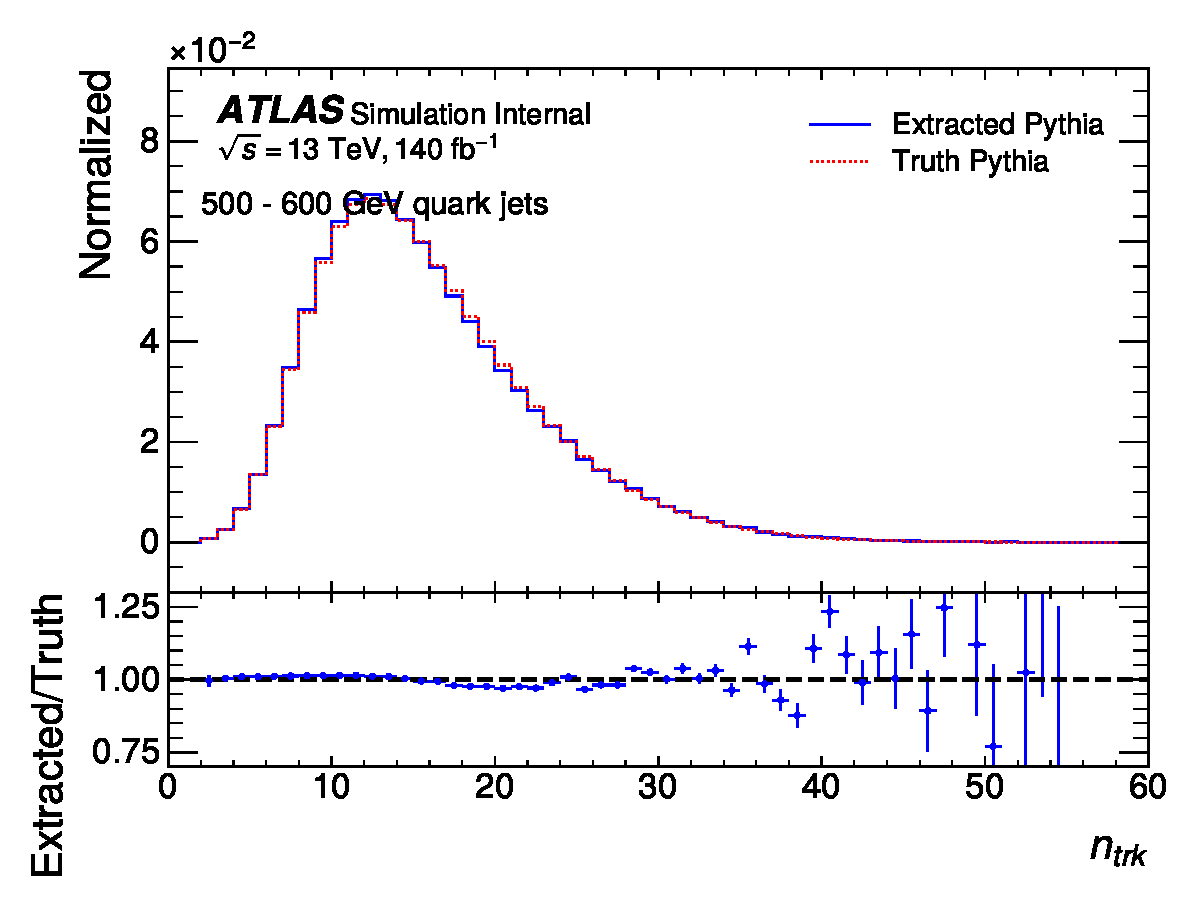
\includegraphics[width=0.45\textwidth]{fig/ADE/MCClosure/jet_nTracks_quark_reweighting_weights/jet_nTracks/MCClosure_500_quark_jet_nTracks.pdf}} \quad
	\subfloat[ ]{\label{fig:QG-pythia-GluonNtrkMCExtractedQuarkFactor-Ntrk-500-600-Ntrk}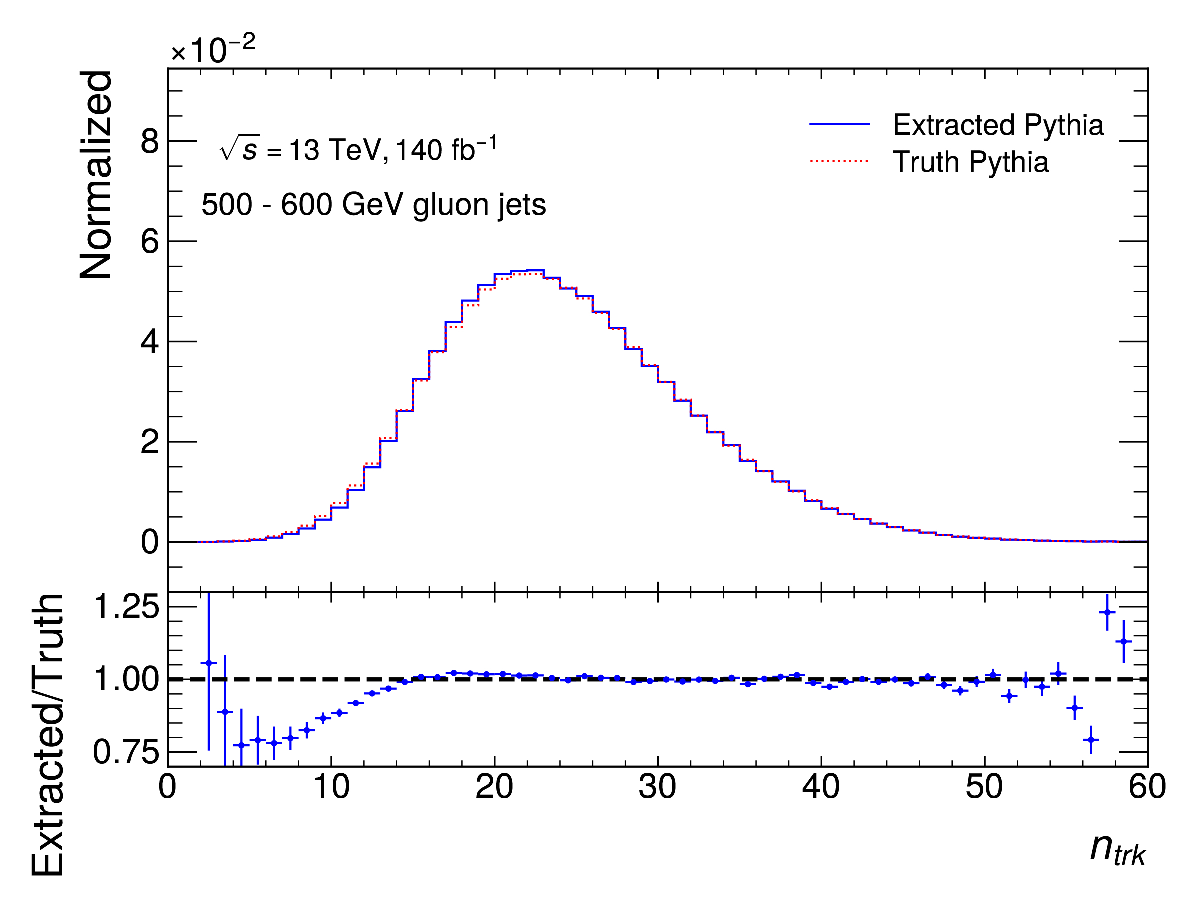
\includegraphics[width=0.45\textwidth]{fig/ADE/MCClosure/jet_nTracks_quark_reweighting_weights/jet_nTracks/MCClosure_500_gluon_jet_nTracks.pdf}} \\
	\subfloat[ ]{\label{fig:QG-pythia-QuarkNtrkMCExtractedEQuarkFactor-Ntrk-800-1000-Ntrk}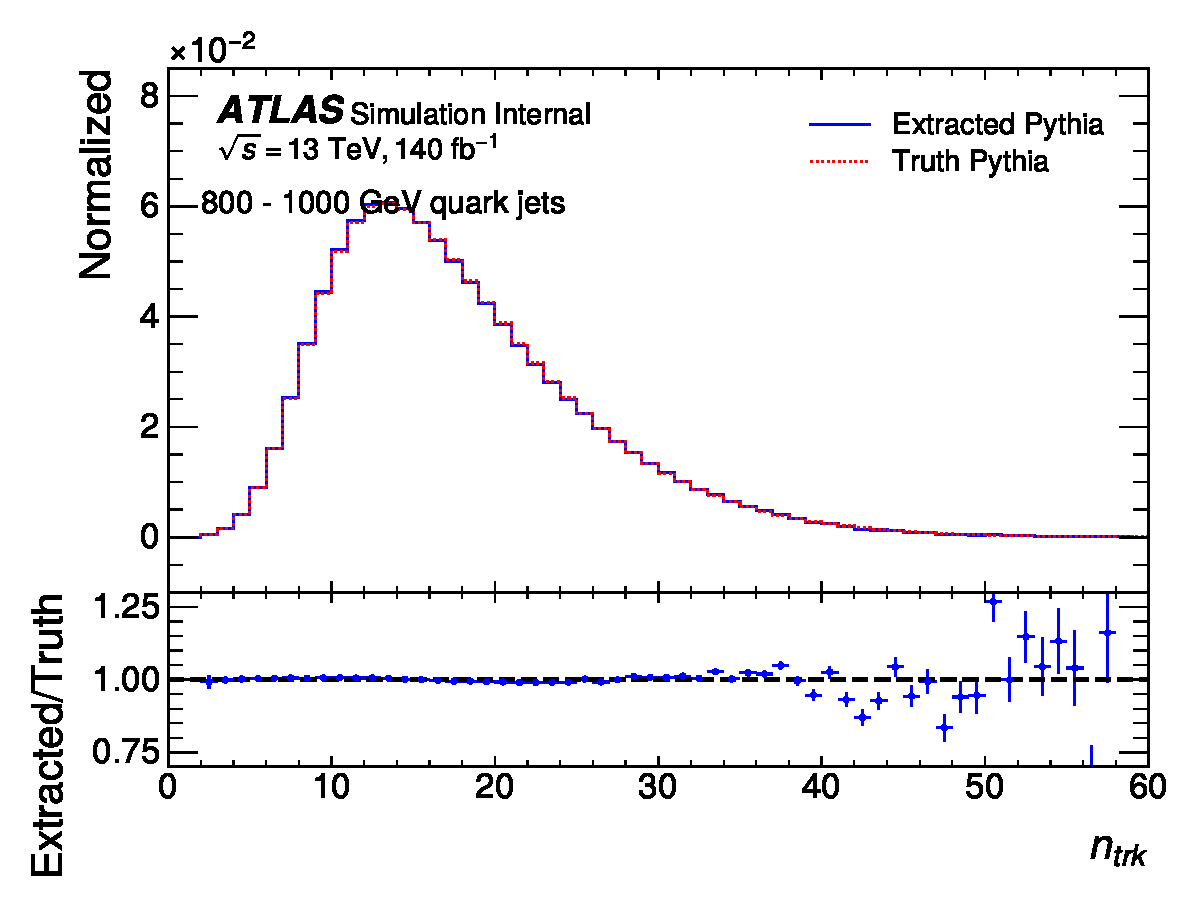
\includegraphics[width=0.45\textwidth]{fig/ADE/MCClosure/jet_nTracks_quark_reweighting_weights/jet_nTracks/MCClosure_800_quark_jet_nTracks.pdf}} \quad
	\subfloat[ ]{\label{fig:QG-pythia-GluonNtrkMCExtractedQuDarkFactor-Ntrk-800-1000-Ntrk}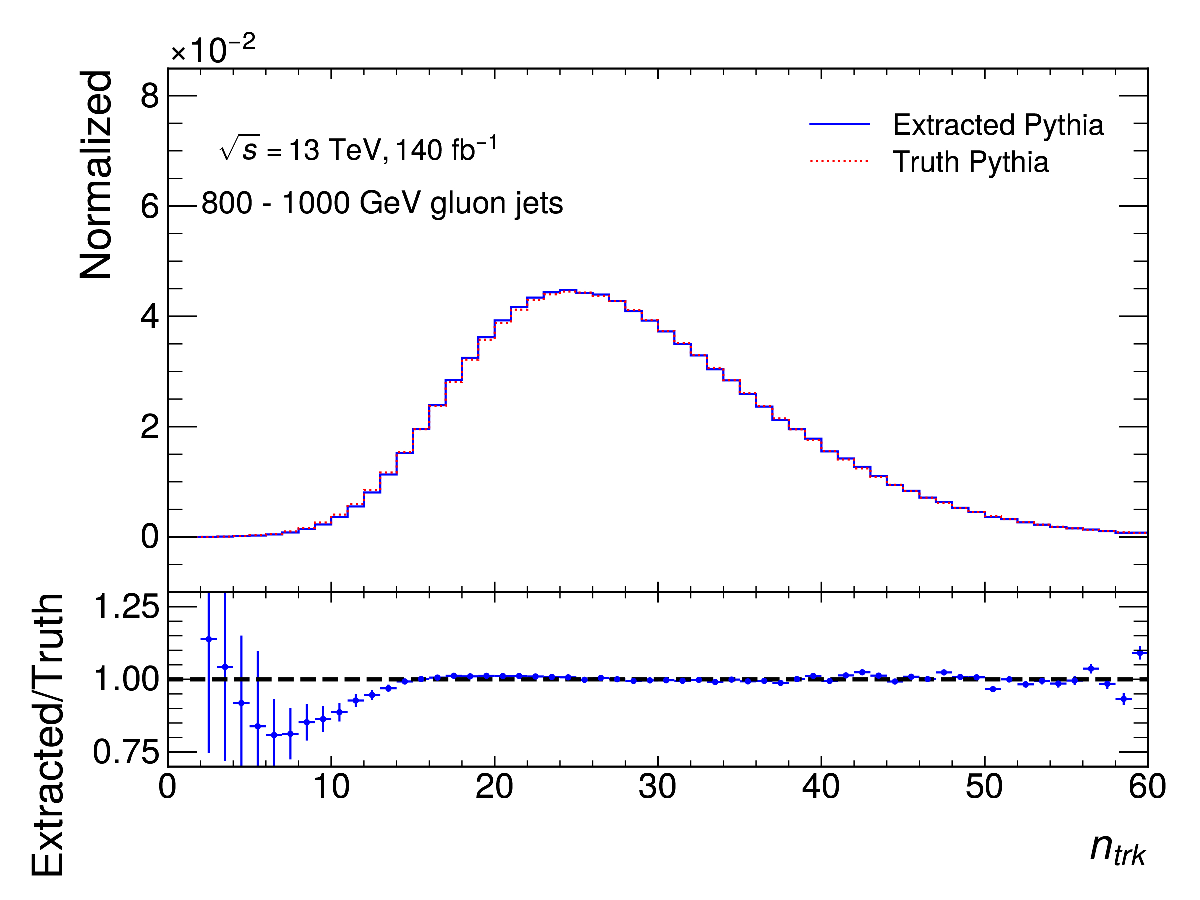
\includegraphics[width=0.45\textwidth]{fig/ADE/MCClosure/jet_nTracks_quark_reweighting_weights/jet_nTracks/MCClosure_800_gluon_jet_nTracks.pdf}} \\
	\caption[]{
		After re-weighting with quark factor: the {\ntrk} distributions of quark-jet \subref{fig:QG-pythia-QuarkNtrkMCExtractedQuarkFactor-Ntrk-500-600-Ntrk} \subref{fig:QG-pythia-QuarkNtrkMCExtractedEQuarkFactor-Ntrk-800-1000-Ntrk} 
		and gluon-jet in \subref{fig:QG-pythia-GluonNtrkMCExtractedQuarkFactor-Ntrk-500-600-Ntrk} \subref{fig:QG-pythia-GluonNtrkMCExtractedQuDarkFactor-Ntrk-800-1000-Ntrk}
		 from {\pythia8} sample. %
		Dashed and solid-line show the {\ntrk} distributions in the truth MC and extracted MC, respectively.
		Bottom panels show the ratio of the extracted MC to the truth MC. %
		\label{fig:QG-pythia-NtrkMCExtractedQuarkFactor-Ntrk}
	}
\end{figure}

\FloatBarrier

\subsubsection{Closure test for BDT tagger}
Similar to the distribution of {\ntrk}, the distributions of BDT score for truth labelled-jets exhibit systematic disparities in forward and central regions. Therefore, the same re-weighting procedure as described is performed for BDT tagger as well. The MC non-closure test is thus conducted by comparing the distributions of BDT score for extracted and truth quark- and gluon-jets, separately, as shown in Figure~\ref{fig:QG-pythia-BDTMCExtracted-Reweight-Compare1}. The distributions of BDT before and after re-weighting are shown in Figure~\ref{fig:QG-pythia-BDTMCExtractedNoReweight} and Figure~\ref{fig:QG-pythia-BDTMCExtractedQuarkFactor-BDT}. The non-closure is about few percent level and taken as one systematic uncertainty.

\begin{figure}[htb]
	\centering
	\subfloat[ ]{\label{fig:QG-pythia-BDTMCExtractedNoreweight-500-600-BDT}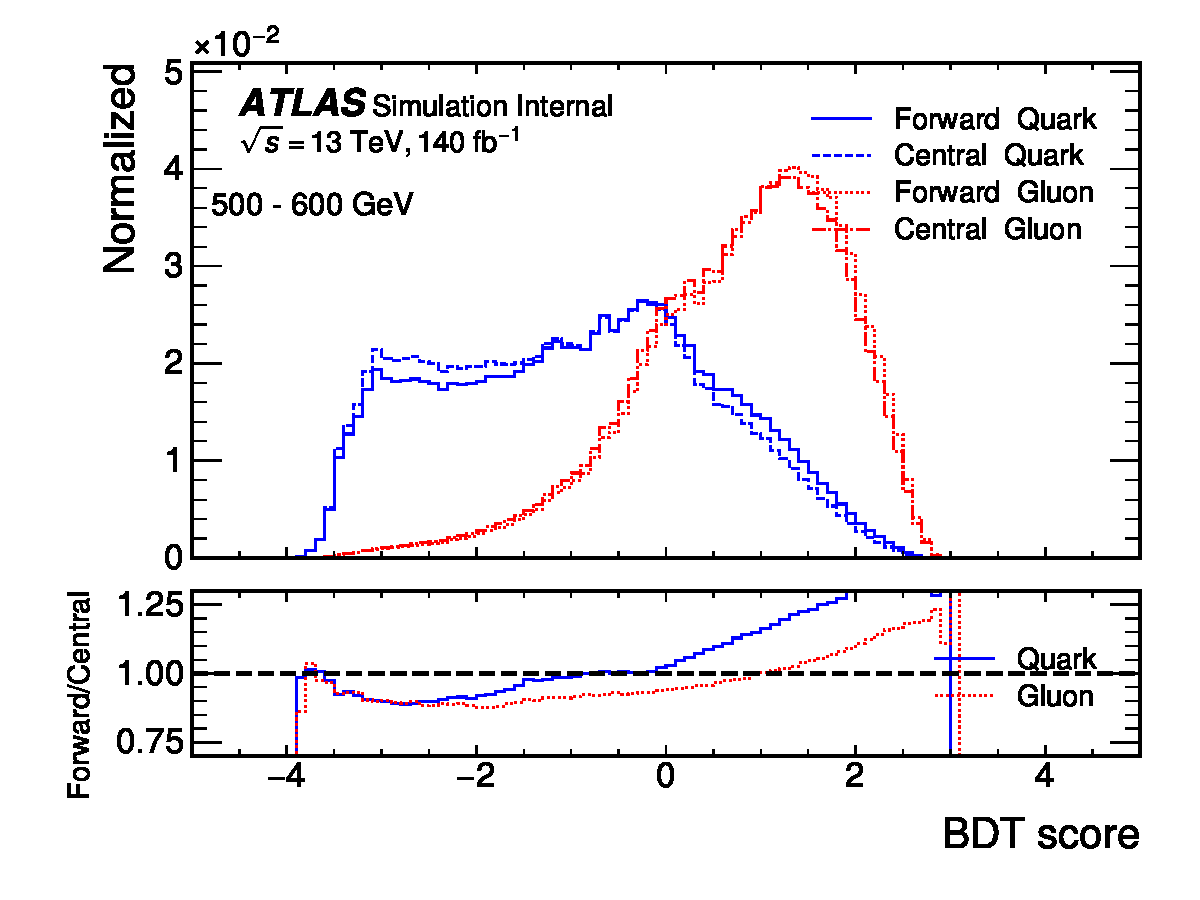
\includegraphics[width=0.45\textwidth]{fig/ADE/FvsC/none_event_weight/GBDT_newScore/MC_truth_Q_G_FvsC_500_GBDT_newScore_event_weight.pdf}} \quad
	\subfloat[ ]{\label{fig:QG-pythia-BDTMCExtractedQuarkFactor-500-600-BDT}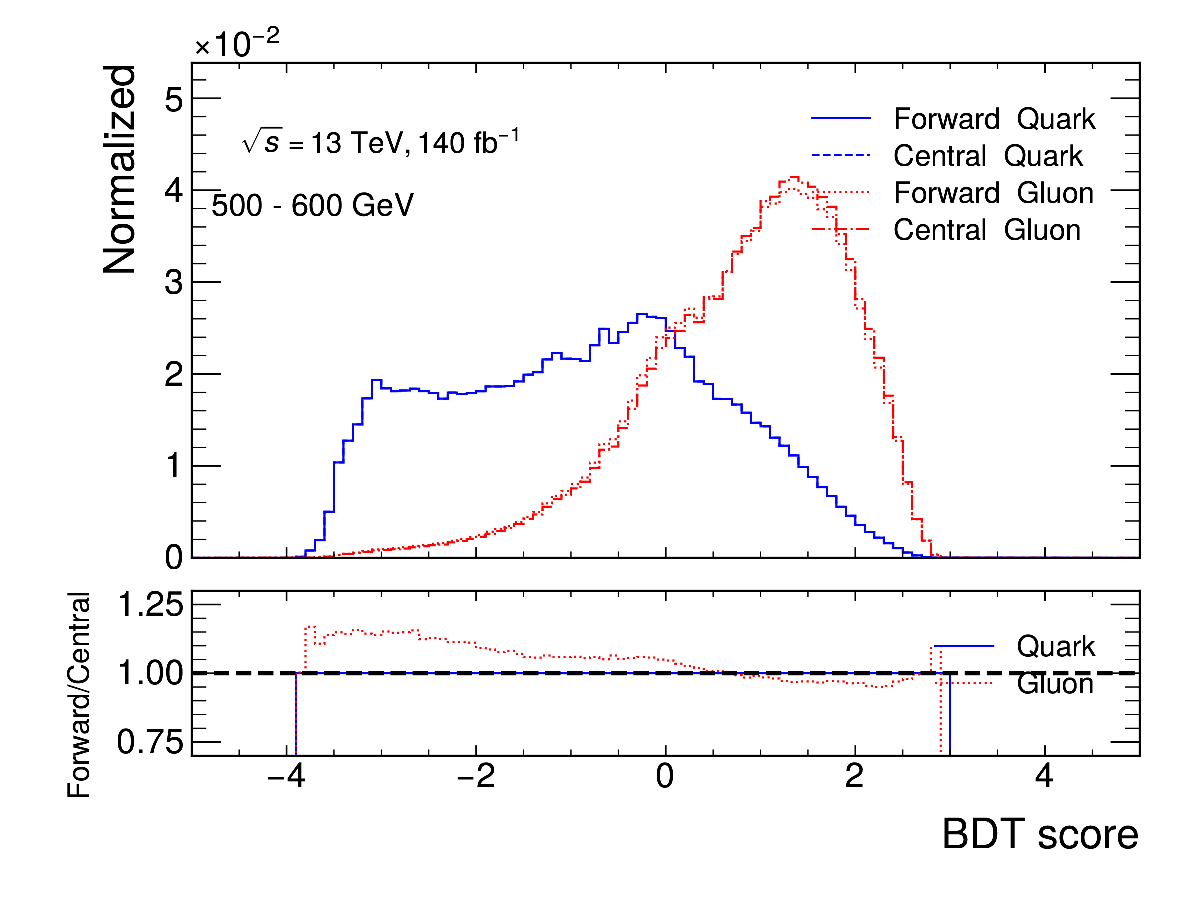
\includegraphics[width=0.45\textwidth]{fig/ADE/FvsC/GBDT_newScore_quark_reweighting_weights/GBDT_newScore/MC_truth_Q_G_FvsC_500_GBDT_newScore_quark_reweighting_weights.pdf}} \\
	\subfloat[ ]{\label{fig:QG-pythia-BDTMCExtractedNoreweight-800-1000-BDT}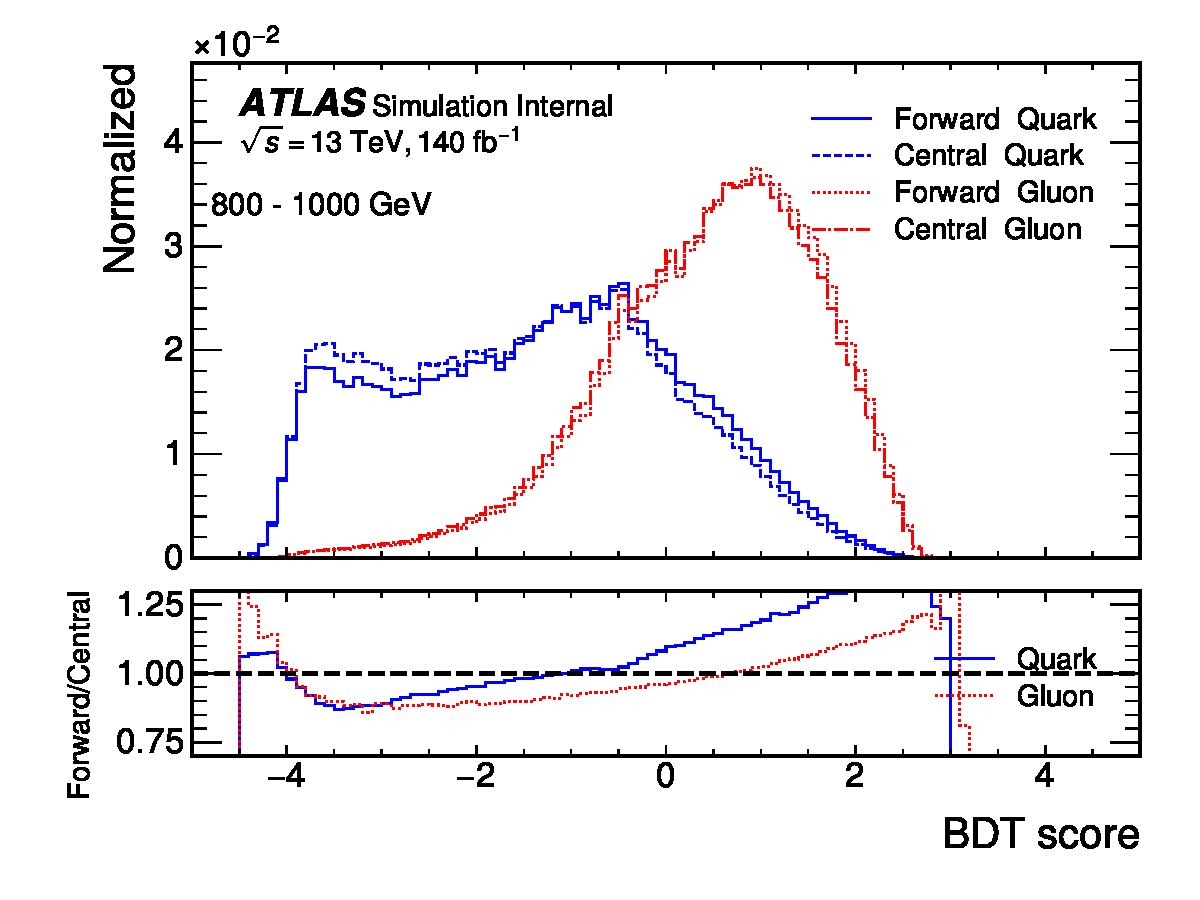
\includegraphics[width=0.45\textwidth]{fig/ADE/FvsC/none_event_weight/GBDT_newScore/MC_truth_Q_G_FvsC_800_GBDT_newScore_event_weight.pdf}} \quad
	\subfloat[ ]{\label{fig:QG-pythia-BDTMCExtractedQuarkFactor-800-1000-BDT}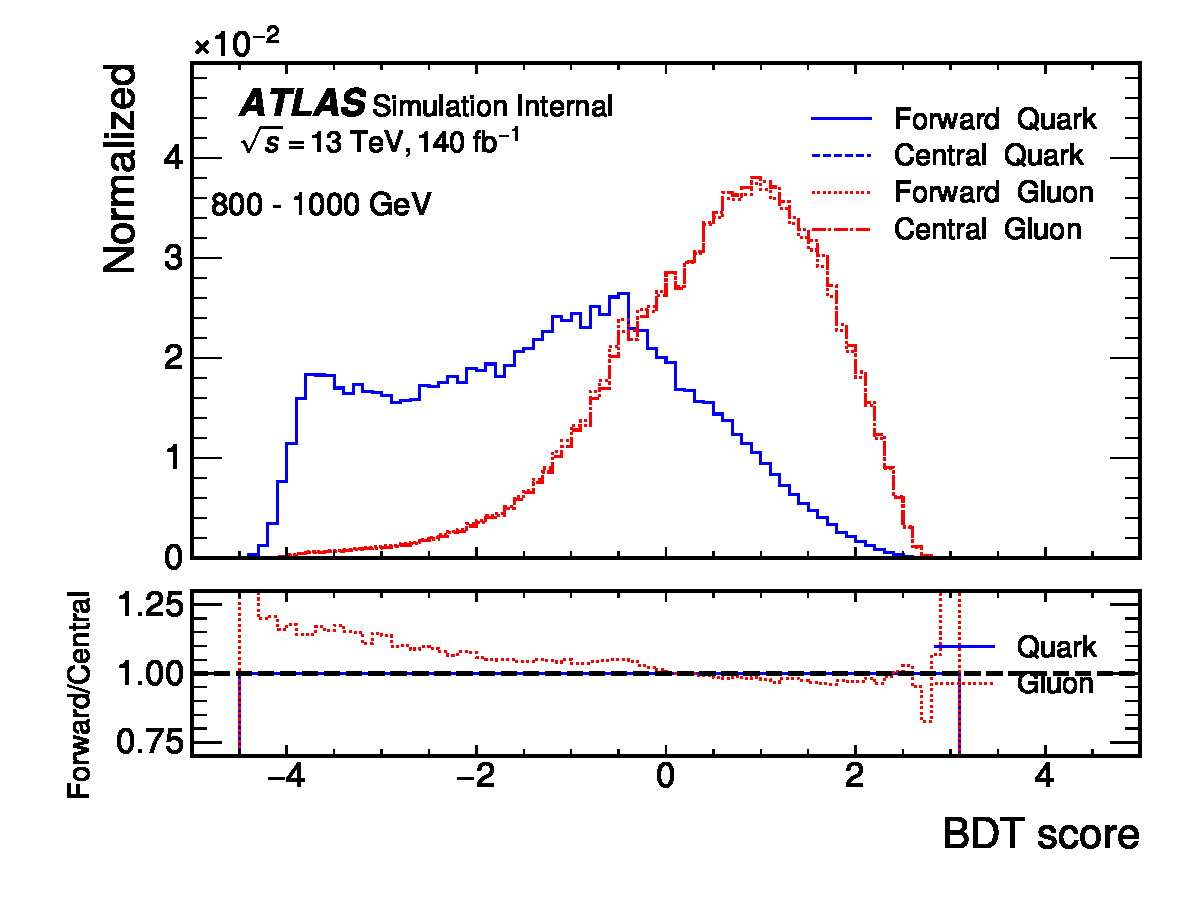
\includegraphics[width=0.45\textwidth]{fig/ADE/FvsC/GBDT_newScore_quark_reweighting_weights/GBDT_newScore/MC_truth_Q_G_FvsC_800_GBDT_newScore_quark_reweighting_weights.pdf}} \\
	\caption[]{
		The distribution of BDT score for jets
		before \subref{fig:QG-pythia-BDTMCExtractedNoreweight-500-600-BDT} \subref{fig:QG-pythia-BDTMCExtractedNoreweight-800-1000-BDT} and 
		after \subref{fig:QG-pythia-BDTMCExtractedQuarkFactor-500-600-BDT} \subref{fig:QG-pythia-BDTMCExtractedQuarkFactor-800-1000-BDT} re-weighting. 
		\label{fig:QG-pythia-BDTMCExtracted-Reweight-Compare1}
	}
	
\end{figure}



%
\begin{figure}[htb]
	\centering
	\subfloat[ ]{\label{fig:QG-pythia-QuarkBDTMCExtractedNoReweight-500-600-BDT}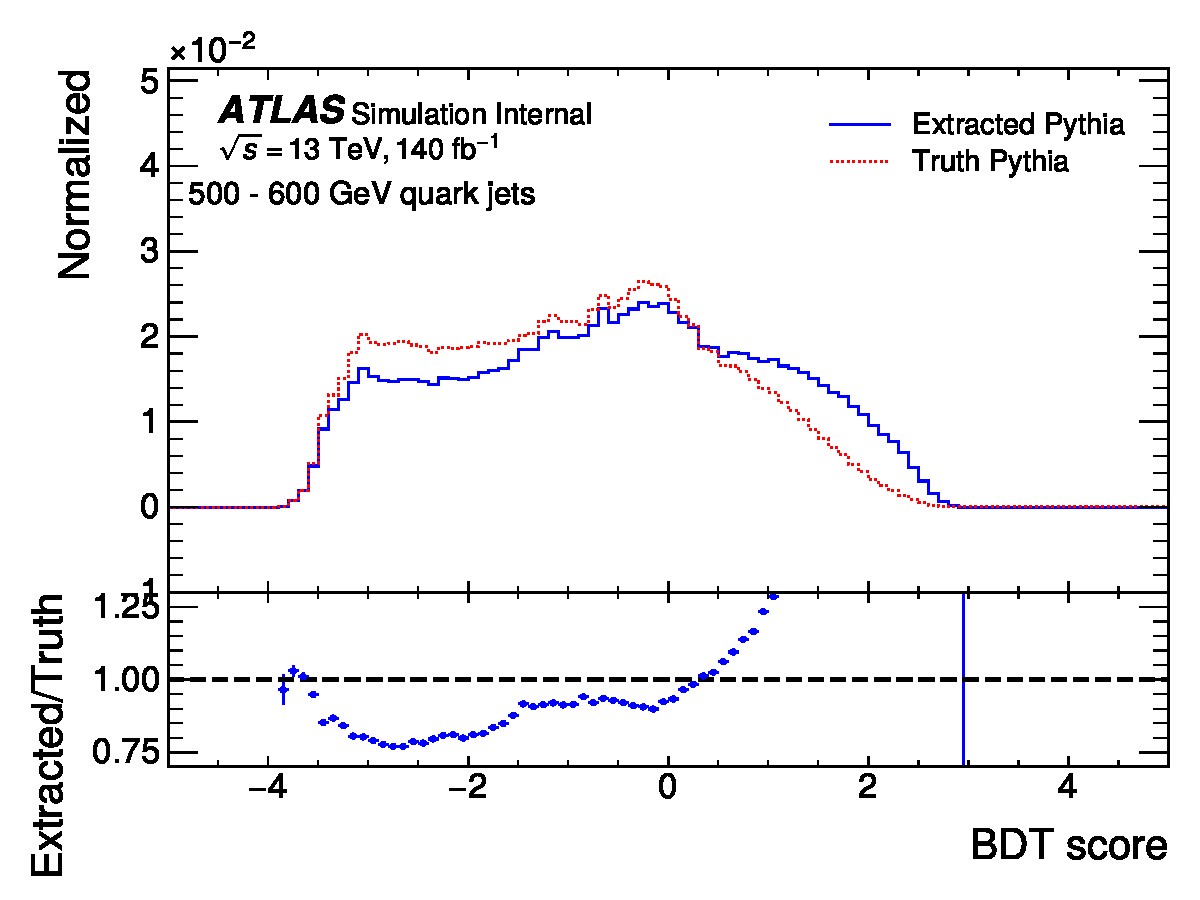
\includegraphics[width=0.45\textwidth]{fig/ADE/MCClosure/none_event_weight/GBDT_newScore/MCClosure_500_quark_GBDT_newScore.pdf}} \quad
	\subfloat[ ]{\label{fig:QG-pythia-GluonBDTMCExtractedNoReweight-500-600-BDT}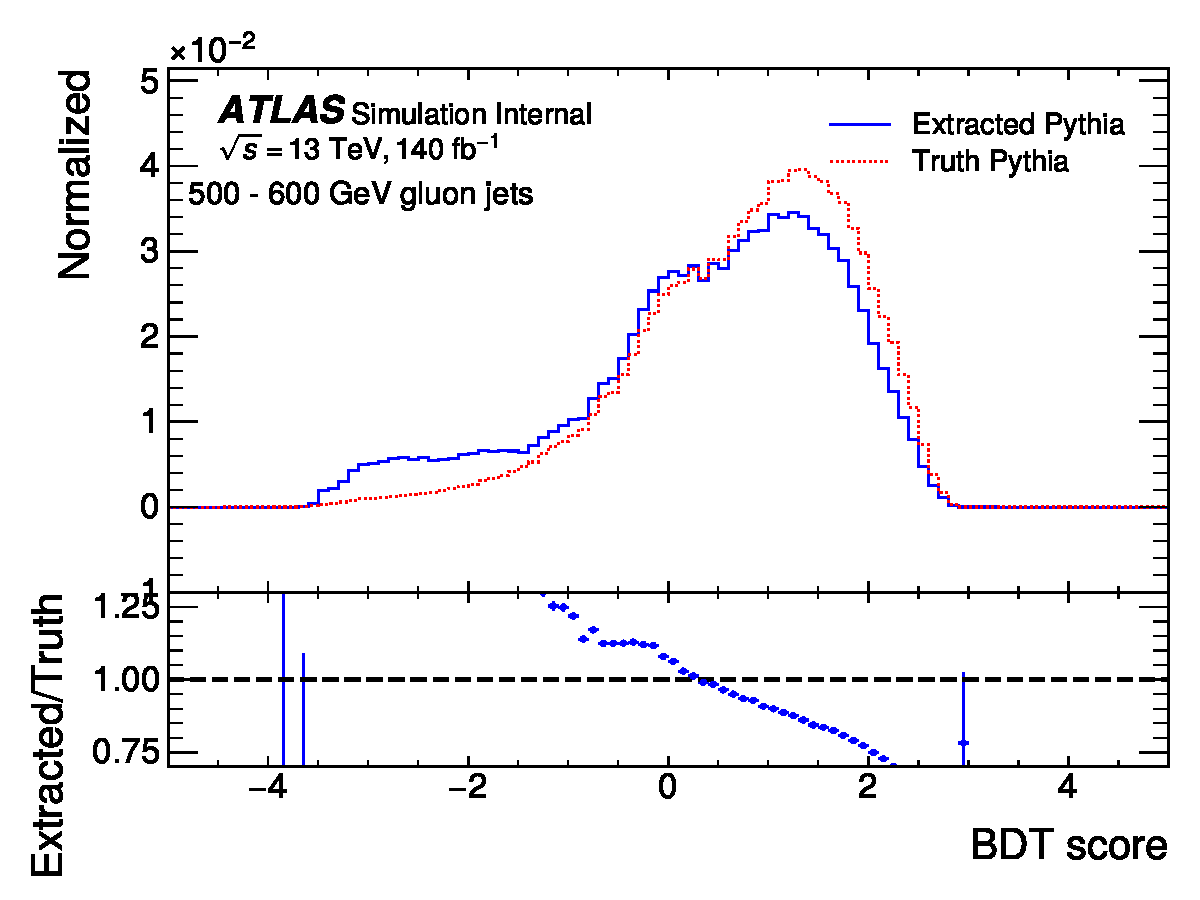
\includegraphics[width=0.45\textwidth]{fig/ADE/MCClosure/none_event_weight/GBDT_newScore/MCClosure_500_gluon_GBDT_newScore.pdf}} \\
	\subfloat[ ]{\label{fig:QG-pythia-QuarkBDTMCExtractedNoReweight-800-1000-BDT}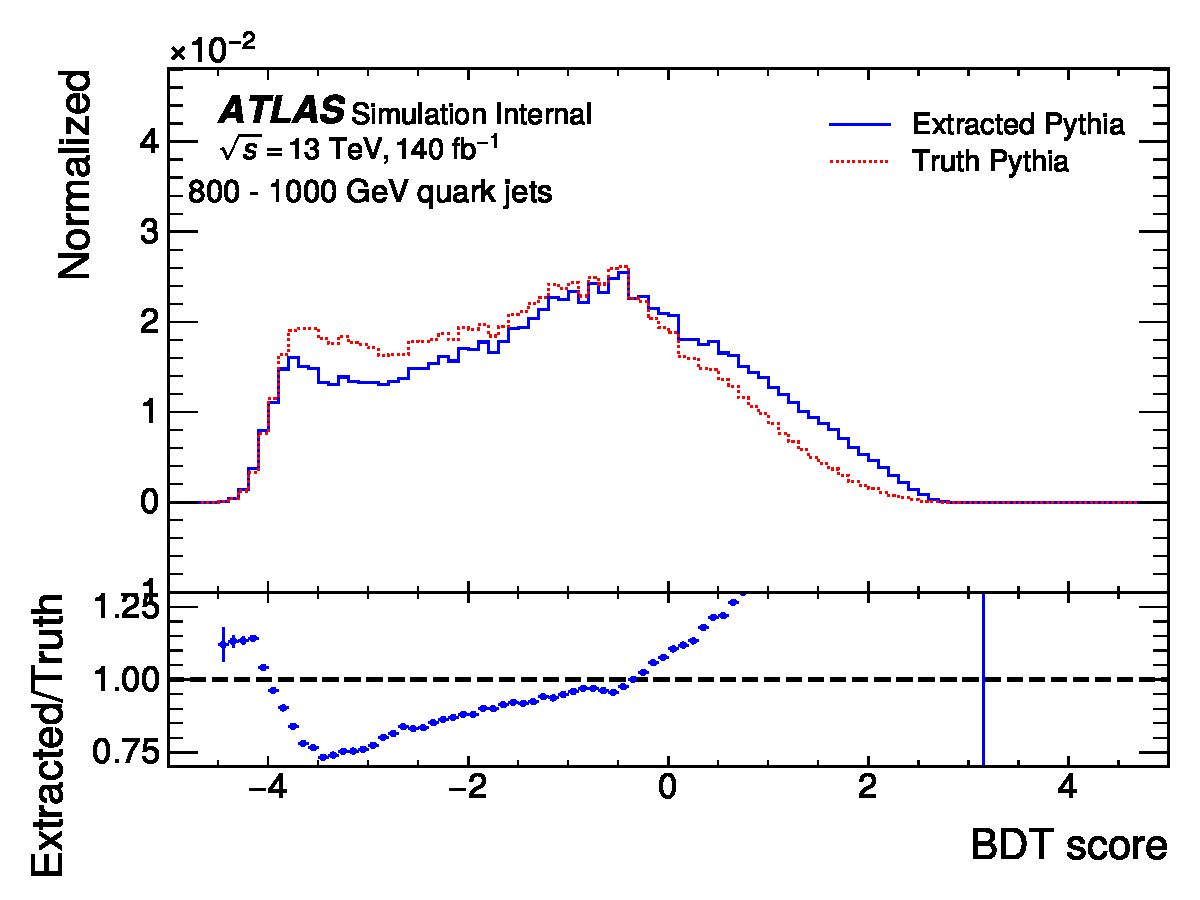
\includegraphics[width=0.45\textwidth]{fig/ADE/MCClosure/none_event_weight/GBDT_newScore/MCClosure_800_quark_GBDT_newScore.pdf}} \quad
	\subfloat[ ]{\label{fig:QG-pythia-GluonBDTMCExtractedNoReweight-800-1000-BDT}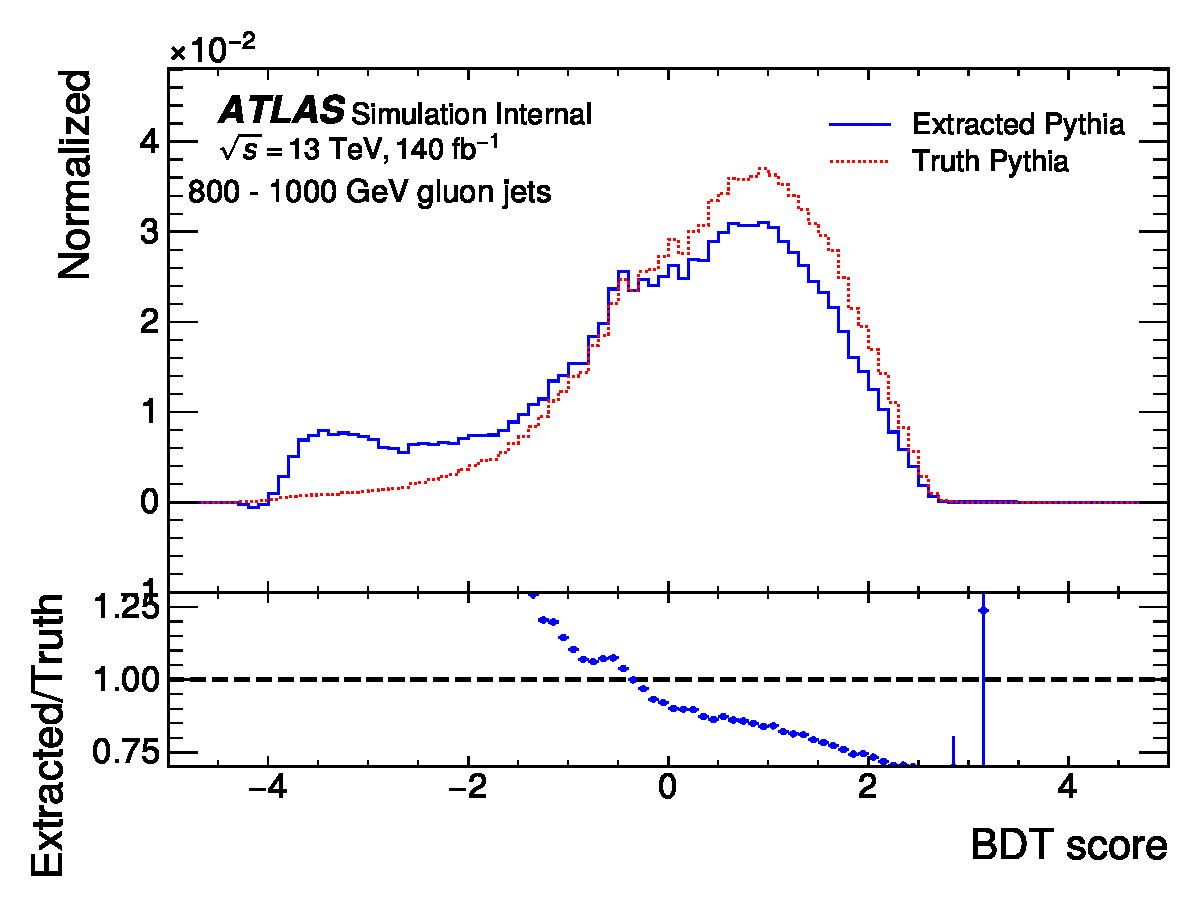
\includegraphics[width=0.45\textwidth]{fig/ADE/MCClosure/none_event_weight/GBDT_newScore/MCClosure_800_gluon_GBDT_newScore.pdf}} \\
	\caption[]{
		Before re-weighting: the MC-closure for quark-jet in \subref{fig:QG-pythia-QuarkBDTMCExtractedNoReweight-500-600-BDT} \subref{fig:QG-pythia-QuarkBDTMCExtractedNoReweight-800-1000-BDT}  
		and for gluon-jet in \subref{fig:QG-pythia-GluonBDTMCExtractedNoReweight-500-600-BDT}  \subref{fig:QG-pythia-GluonBDTMCExtractedNoReweight-800-1000-BDT} 
		in BDT distributions from {\pythia8} sample. %
		Dashed and solid-line histograms show the BDT distributions in the truth MC and extracted MC, respectively.
		Bottom panels show the ratio of the extracted MC to the truth MC. %
		\label{fig:QG-pythia-BDTMCExtractedNoReweight}
	}
\end{figure}



\begin{figure}[htb]
	\centering
	\subfloat[ ]{\label{fig:QG-pythia-QuarkBDTMCExtractedQuarkFactor-BDT-500-600-BDT}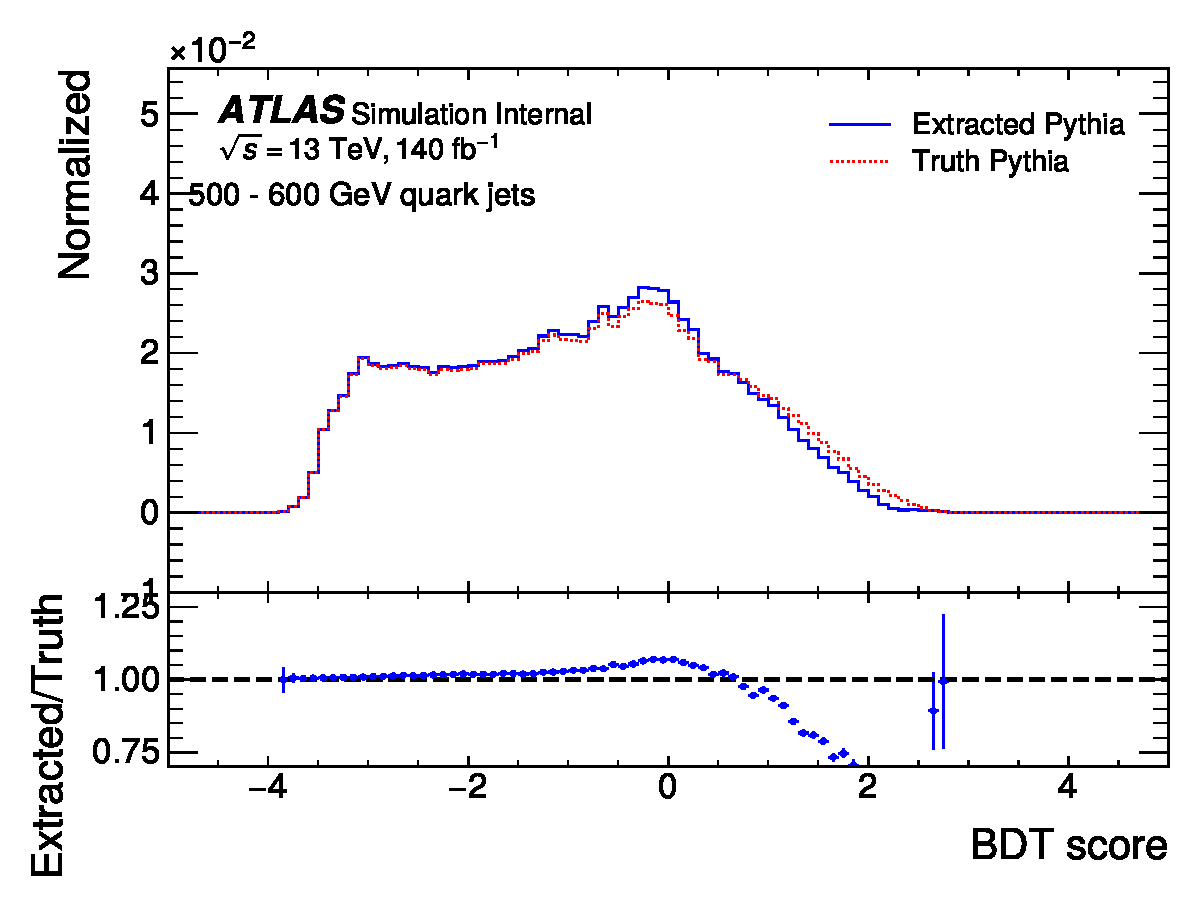
\includegraphics[width=0.45\textwidth]{fig/ADE/MCClosure/GBDT_newScore_quark_reweighting_weights/GBDT_newScore/MCClosure_500_quark_GBDT_newScore.pdf}} \quad
	\subfloat[ ]{\label{fig:QG-pythia-GluonBDTMCExtractedQuarkFactor-BDT-500-600-BDT}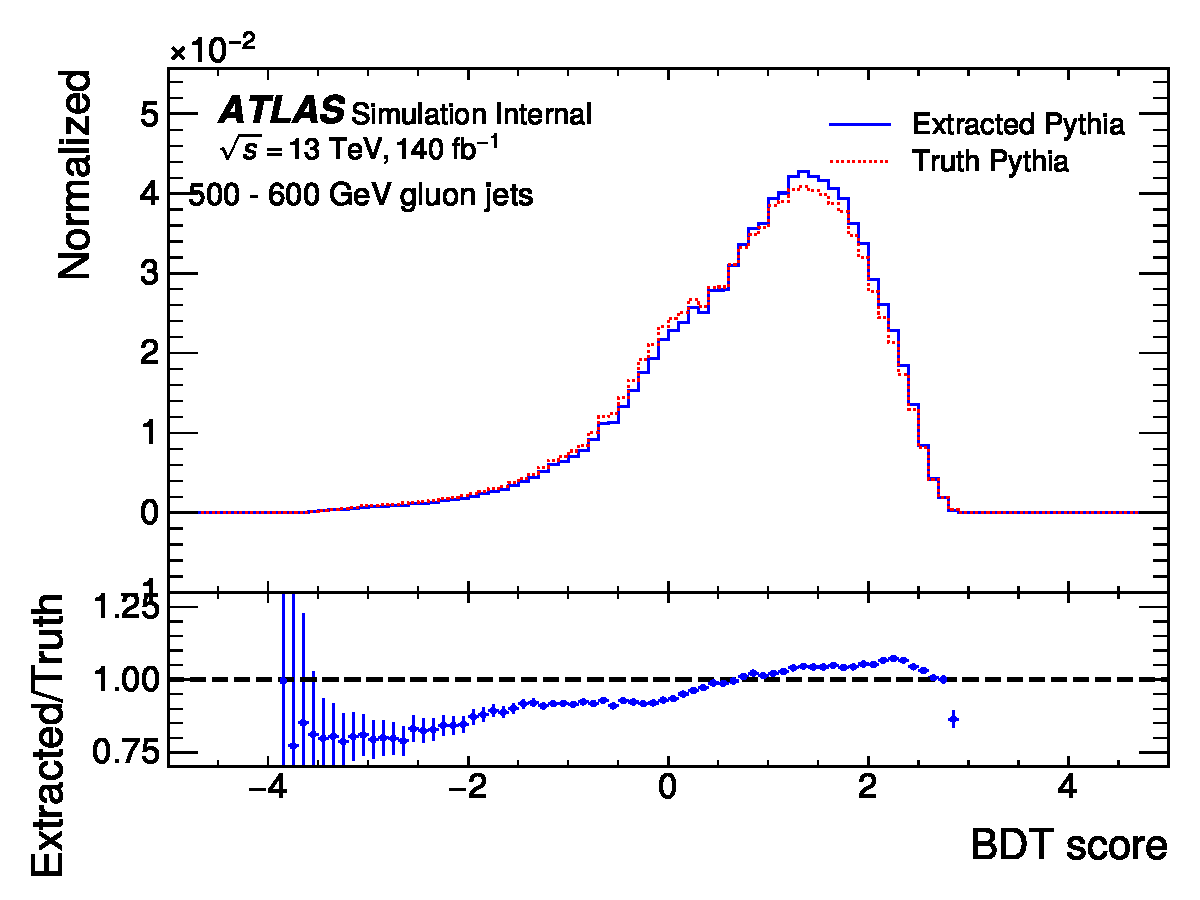
\includegraphics[width=0.45\textwidth]{fig/ADE/MCClosure/GBDT_newScore_quark_reweighting_weights/GBDT_newScore/MCClosure_500_gluon_GBDT_newScore.pdf}} \\
	\subfloat[ ]{\label{fig:QG-pythia-QuarkBDTMCExtractedQuarkFactor-BDT-800-1000-BDT}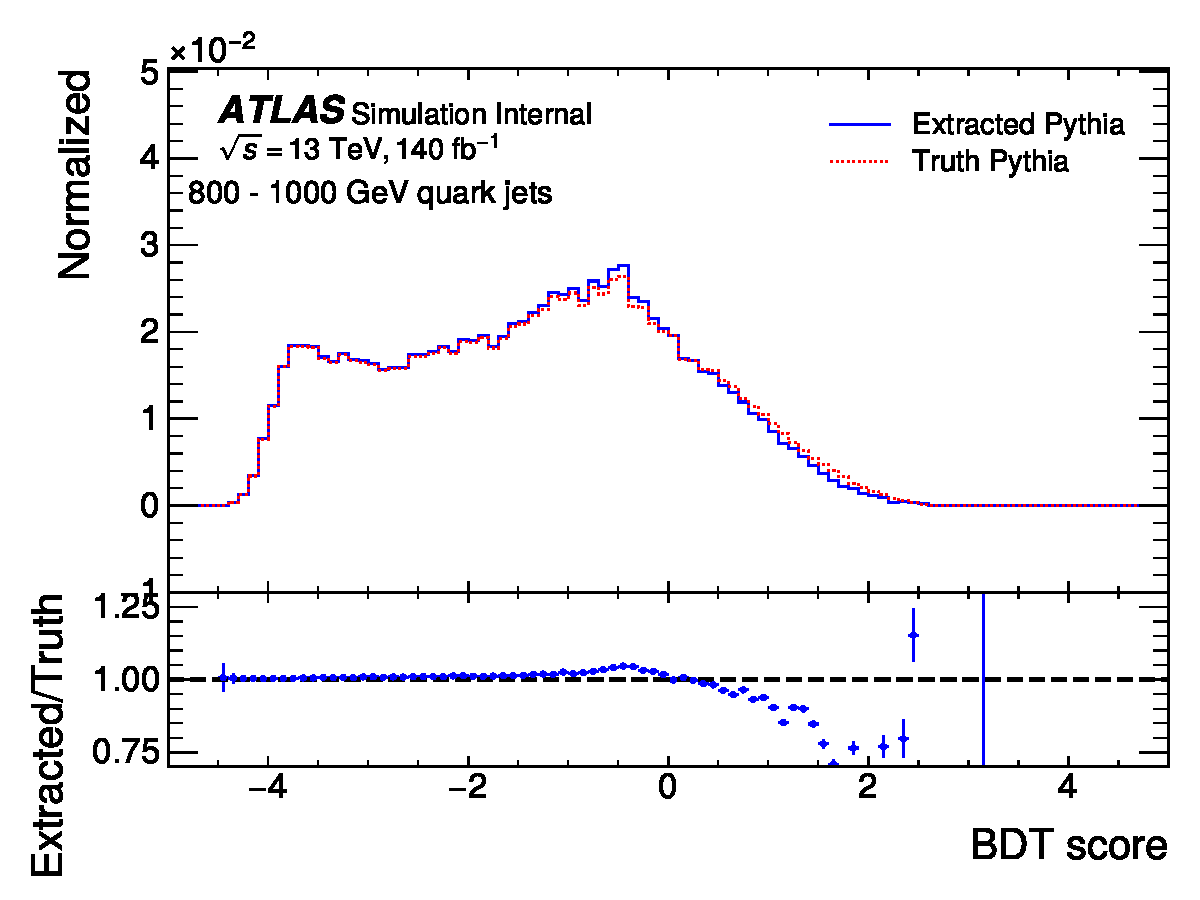
\includegraphics[width=0.45\textwidth]{fig/ADE/MCClosure/GBDT_newScore_quark_reweighting_weights/GBDT_newScore/MCClosure_800_quark_GBDT_newScore.pdf}} \quad
	\subfloat[ ]{\label{fig:QG-pythia-GluonBDTMCExtractedQuarkFactor-BDT-800-1000-BDT}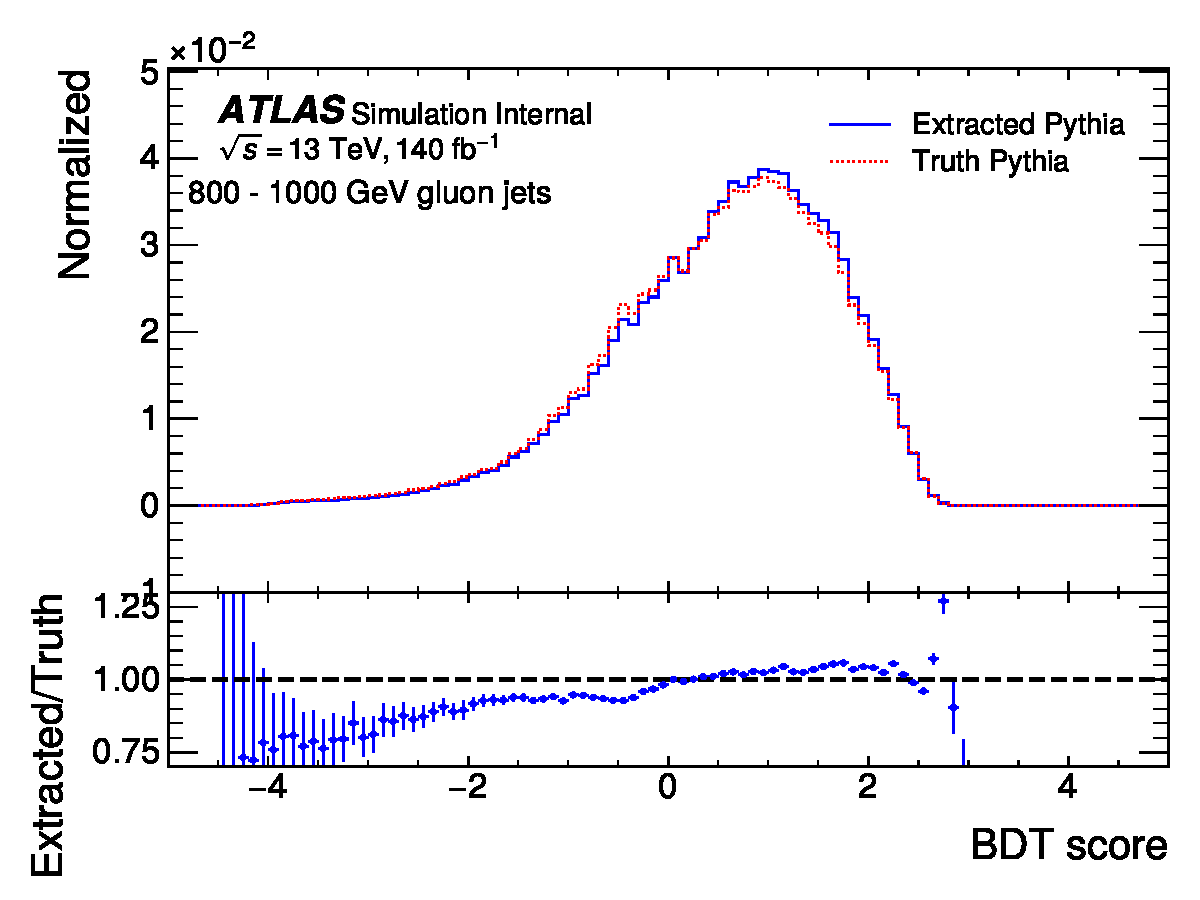
\includegraphics[width=0.45\textwidth]{fig/ADE/MCClosure/GBDT_newScore_quark_reweighting_weights/GBDT_newScore/MCClosure_800_gluon_GBDT_newScore.pdf}} \\
	\caption[]{
		After re-weighting: the MC-closure for quark-jet in \subref{fig:QG-pythia-QuarkBDTMCExtractedQuarkFactor-BDT-500-600-BDT} \subref{fig:QG-pythia-QuarkBDTMCExtractedQuarkFactor-BDT-800-1000-BDT} 
		and for gluon-jet in \subref{fig:QG-pythia-GluonBDTMCExtractedQuarkFactor-BDT-500-600-BDT}  \subref{fig:QG-pythia-GluonBDTMCExtractedQuarkFactor-BDT-800-1000-BDT} in BDT distributions from {\pythia8} sample. %
		Dashed and solid-line histograms show the BDT distributions in the truth MC and extracted MC, respectively.
		Bottom panels show the ratio of the extracted MC to the truth MC. %
		\label{fig:QG-pythia-BDTMCExtractedQuarkFactor-BDT}
	}
\end{figure}





\FloatBarrier

\subsubsection{Summary for the MC Closure test}
\label{sec:mcclosure-summary}
After applied the re-weighting factor to the jet tagging variables {\ntrk} and BDT, the distributions of extracted quark-and gluon-jets converge with those of truth jets. The residual discrepancy, which has only few percent level to the total events is taken into account as MC non-closure systematic uncertainty. No obvious dependency on jet $\eta$ is observed from the distributions of jet tagging variables.

